\chapter{Introduction}\label{chap:Intro}

\section{Problématiques}
Les problèmes d'inter-opérabilité et de réutilisabilité font partie des problématiques majeures des systèmes informatiques. La programmation objet ne parvient pas à répondre à ces problématiques à cause notamment de ses propriétés de granularité et de fort couplage. Les problèmes de cohésions (pas d'explications des besoins requis) sont aussi un frein à l'utilisation de la programmation objet à grande échelle. 

Parmi les solutions à ces problématiques les architectures à composants sont des alternatives efficaces. Un composant, entité principale, correspond par définition à une ou plusieurs fonctionnalités. Il est donc possible de le concevoir et de le pré-tester de manière indépendante. La coopération entre composant est alors plus aisée. De plus un composant possède un couplage lâche. Cette propriété garantissant l'inter-opératibilté est permise par l'utilisation d'interfaces entre composant. 

\section{Présentation du sujet}
Le module \textsc{Architectures and Components} nous propose une étude de la programmation par composants. L'objectif de ce projet/TP  est de réaliser un \textsc{Home Architecture Description Language}, et d'implémenter une architecture classique \emph{Clients-Serveur}. La démarche proposée pour atteindre cet objectif est composée de trois étape : 


\begin{enumerate}
\item 
  Réalisation du M2 :\hfill \\
  Il s'agit d'un méta-modèle de l'architecture de composants.  
\item
  Réalisation du M1 :\hfill \\
  À partir du méta-modèle précédement réalisé, nous pouvons proposer une instance de ce dernier et obtenir un modèle. Nous choisirons ici de modéliser une application classique \emph{Clients-Serveur}.  
\item
  Réalisation du M0 :\hfill \\
  Dernière étape, elle consiste en l'instanciation concrêtes des classes décrites dans le M1.
\end{enumerate}

\clearpage

\section{Rappel du modèle à composants}
Dans cette partie nous rappelerons les différents éléments du modèle à composants ainsi que leur(s) fonctionnalité(s).

\begin{description}
\item[Composant] \hfill \\
  Un composant est une unité de composition qui spécifie  une ou plusieurs fonctionnalités. Les composants fournissent des services et requièrent des besoins. Ils peuvent être déployés (installés) indépendamment et composés avec d'autres composants.
  \begin{figure}[htb]
    \centering
    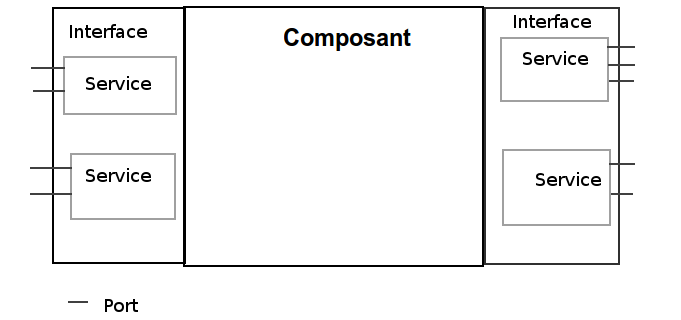
\includegraphics[scale=0.36]{img/composant}
    \caption{Exemple de composant}
    \label{fig:compo}
  \end{figure}
  
  Il sont préfabriqués, pré-testés et s'autocontiennent. Ils sont configurables et sont capables d'user de mécanismes d'introspection qui leurs permettent de connaître et de modifier leurs caractéristiques.
\item[Interfaces] \hfill \\
  Ce sont les seules parties visibles d'un composant. Elles sont constituées de ports (ou points de connexions) et de services.
\item[Ports]\hfill \\
  Ils permettent la communication entre composants. Un port peut être requis ou fourni.  
\item[Services] \hfill \\ Un service est soit une fonctionnalité offerte soit une fonctionnalité demandée  par le composant. Un service est associé à un certain nombre de ports requis et fournis. Un exemple de composant est proposé sur la figure \ref{fig:compo}.
\item[Propriétés] \hfill \\  Elle peuvent concerner aussi bien la structure que le comportement d'un composant et sont paramétrables. Elles peuvent être :
  \begin{itemize}
  \item 
    Fonctionnelles : Une propriété relative au fonctionnement du composant.
  \item 
    Non fonctionnelles : Une propriété indépendante du fonctionnement telle que la sécurité ou la performance.
  \end{itemize}
\item[Connecteurs] \hfill \\
  Ils permettent de connecter deux composants entre eux au niveau de leurs ports, permettant la communication entre un service fourni et un service requis. Le fonctionnement d'un connecteur est implémenté par la glu. Il est cependant possible qu'un connecteur soit implémenté par une configuration.
\item[Glu] \hfill \\
  Elle définit le fonctionnement du connecteur.
\item[Rôle] \hfill \\
  Un rôle est l'élément permettant de relier un connecteur aux ports d'un composant.
\item[Attachement] \hfill \\
  Il permet la liaison entre les ports d'un composant et un rôle d'un connecteur.
\item[Configuration] \hfill \\
  La configuration est un composant composé de composants (Design pattern \emph{Composite}).
\item[Binding] \hfill \\
  Il s'agit d'un lien permettant de rediriger des ports d'un composant vers ceux de sa configuration.

\end{description}
